\documentclass[output=paper]{LSP/langsci} 
\author{Letícia M. Sicuro Corrêa\affiliation{Pontifícia Universidade Católica do Rio de Janeiro, Laboratório de Psicolinguística e Aquisição da Linguagem (LAPAL)}\lastand 
Marina R. A. Augusto\affiliation{Universidade do Estado do Rio de Janeiro, Laboratório de Psicolinguística e Aquisição da Linguagem (LAPAL)}
}
\title{Primeiros passos na aquisição da sintaxe: o sintagma nominal}  
\abstract{}
\ChapterDOI{10.5281/zenodo.889427}
\maketitle
\begin{document}
\section{Introdução} 
\label{sec:correanp_intro}

A aquisição da sintaxe torna-se evidente quando a criança começa a combinar duas ou mais palavras em enunciados aos quais se atribui um sentido. Crianças, não importa a língua que estejam a adquirir, seguem um curso de desenvolvimento comum, compondo enunciados cada vez mais complexos (cf. \citealt{bowerman1973}). Quando se pensa na aquisição da sintaxe, podemos, então, considerar o curso natural por que passam crianças na aquisição de qualquer língua humana, em função de um programa biológico, o qual possibilita a combinação de unidades de um léxico em estruturas nas quais esses elementos se relacionam de forma hierárquica.

Cada língua possui um léxico e durante o primeiro ano de vida a criança extrai dos dados da fala ``pistas” que lhe permitam ``recortar'' o fluxo da fala a ela dirigida e à sua volta, em unidades que possibilitem a identificação de unidades lexicais. Os elementos do léxico das diferentes línguas se distinguem não só no que diz respeito às suas propriedades fonológicas (sua forma fônica) e às suas propriedades semânticas (que podem decorrer de diferentes recortes de ordem conceptual). Variam também em suas propriedades sintáticas, que dizem respeito ao modo como estes se combinam de forma estruturada em enunciados. Nesse sentido, os primeiros passos na aquisição da sintaxe irão refletir não só o desdobramento do programa biológico comum, mas o resultado de um processo de identificação do que há de específico em uma dada língua, a partir dos dados da fala que à criança se apresentam.

Este capítulo tem como foco os primeiros passos desse processo, no que concerne ao que tradicionalmente é denominado \textit{sintagma nominal}.\is{sintagma nominal} Sintagmas ou constituintes oracionais são unidades sintáticas que compõem a estrutura hierárquica de sentenças\footnote{``Sentença'' é o termo utilizado, no Brasil, particularmente por linguistas de orientação generativista, como equivalente ao que a gramática tradicional denomina ``período'' e ``oração''. ``Sentença'' e ``oração'' podem, contudo, ser utilizados de forma intercambiada, ou a utilização de um ou de outro pode ser preferida em alguns contextos ou expressões (ex. Oração principal, oração relativa, sentenças simples e complexas). } das línguas naturais. O prefixo grego\il{grego} \textit{sin-} (que significa ``junto com'', ``ao mesmo tempo''), também presente em sintaxe, indica tratar-se de unidades cujos elementos se relacionam entre si e/ou que se juntam a outras, compondo, desse modo, unidades maiores. Sintagmas podem ser constituídos de um ou mais elementos, com um núcleo, pertencente a uma dada categoria do léxico. O núcleo projeta suas propriedades sintáticas a um nó dominante na estrutura criada. Em (\ref{ex:correanp_1}), A é um núcleo não ramificado, que projeta suas propriedades para uma camada mais alta A’. Em (\ref{ex:correanp_2}), A é um núcleo que se combina com B e o tem como seu complemento. Tem-se, então uma estrutura em que A projeta suas propriedades sintáticas para o nó A’, que domina A e B. Em (\ref{ex:correanp_3}), C é um núcleo que toma A’ como seu complemento. Tem-se, então uma estrutura em que C projeta suas propriedades sintáticas para o nó C’, que domina C e A’.

\ea\label{ex:correanp_1}
\begin{forest} baseline
	[A'[A]]
\end{forest}
\z

\ea\label{ex:correanp_2}
\begin{forest} baseline
	[A'
    	[A]
        [B]
       ]
\end{forest}
\z

\ea\label{ex:correanp_3}
\begin{forest} baseline
	[C'
    	[C]
        [A'
        	[A]
            [B]
        ]
       ]
\end{forest}
\z

Toda sentença pode ser descrita em seus constituintes básicos, ou seja, as unidades sintagmáticas definidas a partir do elemento nuclear que as compõe. Tradicionalmente, os núcleos lexicais, Nome,\is{nome} Verbo, Adjetivo\is{adjetivo} e Preposição foram tomados como os constituintes básicos da oração, formando respetivamente, os sintagmas nominal\is{sintagma nominal} (NP), verbal (VP), adjetival (AdjP) e preposicional (PP).\footnote{Seguimos a convenção de utilizarem-se as siglas originárias do inglês\il{inglês} VP (Verbal Phrase), para sintagma verbal, NP (Noun Phrase) para sintagma nominal,\is{sintagma nominal} PP (Prepositional Phrase) para sintagma preposicional etc.}

Assim, na gramática tradicional, nos primeiros modelos de gramática gerativa,  em descrições gramaticais pouco comprometidas com uma dada teoria linguística, ou mesmo na literatura psicolinguística, de um modo geral, denominam-se sintagmas nominais\is{sintagma nominal} (NPs), os constituintes que ocupam as posições de sujeito, de complemento de verbo (como objeto direto) e de complemento de preposição, com diferentes funções sintáticas (como objeto indireto, complemento nominal, adjunto adnominal, adjunto adverbial). Estes incluem minimamente um nome\is{nome} (comum ou próprio) ou exclusivamente um pronome pessoal, como \textbf{eu, ele/a}, por exemplo. Podem ainda incluir, além do nome,\is{nome} outros elementos como determinantes\is{determinante} (\textbf{a}/\textbf{esta}/\textbf{aquela} menina), adjetivos\is{adjetivo} (a menina \textbf{alta}), sintagmas preposicionais (PP) (a menina \textbf{de chapéu}; a construção \textbf{da cidade}) e orações relativas (o menino \textbf{que chegou}). 

  Diante de uma língua específica, a criança terá de inicialmente delimitar os constituintes nominais no fluxo da fala e sua posição relativa em relação ao verbo, em função da ordem em que se apresentam e da relação semântica que com este mantêm (de argumento interno -- complemento do verbo; ou externo, que assume a posição de sujeito na estrutura da oração). Já internamente, no domínio nominal, a criança terá de identificar os determinantes\is{determinante} que se apresentam, a posição do nome\is{nome} em relação ao determinante,\is{determinante} do adjetivo\is{adjetivo} em relação ao nome,\is{nome} os tipos de distinção conceptual que a língua expressa gramaticalmente em morfemas flexionais, como gênero,\is{género} número,\is{número} no português, distinções de pessoa\is{pessoa} que se fazem visíveis no sistema pronominal, além de distinções sutis, de natureza semântica e referencial como definitude, genericidade, que podem requerer uma sintaxe específica, dentre outras.
  
O domínio \isi{nominal} se faz presente, na fala da criança, desde os primeiros enunciados linguísticos. Substantivos\is{substantivo|see {nome}} (nomes)\is{nome} comuns tendem a ser predominantes em enunciados de uma palavra, independentemente da língua em questão, nomeando objetos, pessoas\is{pessoa} ou classes de elementos de um mesmo tipo \citep{gentnerboroditsky2001}.

As primeiras combinações de palavras trazem uma variedade de possibilidades sugestivas de uma estrutura na qual um constituinte de natureza nominal se faz presente, e em que a ordem das palavras/constituintes da língua já é observada. Os exemplos em (\ref{ex:correanp_4}), extraídos do clássico estudo longitudinal da aquisição do inglês\il{inglês} por três crianças \citep{brown1973}, são ilustrativos do Estádio 1 do desenvolvimento linguístico em uma escala definida pelo número\is{número} de morfemas (MLU – \textit{Mean Length of Utterance}).

\ea\label{ex:correanp_4}
\textit{This train}; \textit{No More};  \textit{Birdie go}; \textit{Push truck}; \textit{Man hat}; \textit{Water hot}; \textit{Kim car}; (MLU 1,75)
\z

Tem-se, em (\ref{ex:correanp_4}), um exemplo de NP pleno (\textit{This car}), elíptico (\textit{No more} X), na forma de nome\is{nome} próprio (\textit{Birdie}),  com estrutura possessiva (\textit{Kim car}), como sujeito (\textit{Birdie go}; \textit{Daddy kiss}), e como complemento de verbo (\textit{push truck}). 

Observações semelhantes podem ser feitas nos dados da fala espontânea de crianças que adquirem diversas línguas, como os registrados no CHILDES,\footnote{CHILDES (\textit{Child Language Data Exchange System}): banco de dados da produção de fala de crianças em diferentes línguas, acessível em \url{http://childes.psy.cmu.edu}.} e em diferentes acervos. No Estádio 2 (MLU 2.25), constata-se, nos dados de Brown, a presença de morfema de concordância\is{concordância} de número\is{número} plural no NP (\textit{my cars}). 

Relações de concordância\is{concordância} decorrem do fato de palavras que se combinam em uma estrutura hierárquica compartilharem traços ou propriedades de natureza sintática (traços formais). O modo como essas relações se expressam na morfologia é, entretanto, algo que a criança tem de perceber e representar na gramática da língua específica que está a adquirir. Em português, por exemplo, a concordância\is{concordância} de número\is{número} (singular; plural) e a concordância\is{concordância} de gênero\is{género} (masculino; feminino) no interior do SN têm, basicamente, expressão morfológica no determinante,\is{determinante} no nome\is{nome} e em adjetivos\is{adjetivo} (\ref{ex:correanp_5}). O gênero\is{género} e o número\is{número} do sujeito da sentença também são, em tese, morfologicamente expressos no predicativo, em construções de cópula (\ref{ex:correanp_6}). Em algumas variantes, a expressão morfológica de número\is{número} pode, não obstante, ficar restrita ao determinante,\is{determinante} estando ausente no nome,\is{nome} em adjetivos\is{adjetivo} (ex. O\textbf{s} menino esperto) e em construções de cópula (ex. O\textbf{s} menino é esperto). 

\ea\label{ex:correanp_5}
O(s)/\textbf{A(s)} menino(s)/\textbf{a(s)} esperto/\textbf{a(s)}. 
\z
\ea\label{ex:correanp_6}
Este\textbf{(s)}/Esta\textbf{(s)} menino(s)/\textbf{a(s)} é(são) esperto\textbf{(s)}/\textbf{a(s)}.
\z

A pessoa\is{pessoa} gramatical do SN sujeito pode ter reflexo na morfologia flexional. Em português, a pessoa\is{pessoa} e o número\is{número} do constituinte nominal sujeito determinam a expressão morfológica de pessoa\is{pessoa} e número\is{número} do verbo, em função da relação de concordância\is{concordância} que se estabelece. Por volta dos dois anos de idade, crianças adquirindo o português fazem distinções entre 1ª e 3ª pessoa\is{pessoa} gramatical que repercutem no verbo (\textit{Quero}/\textit{Quer}, por exemplo) \citep{martins2007}. Em línguas de sujeito nulo, como o português (i.e em que a posição de sujeito pode não ser lexicalmente preenchida como em (\ref{ex:correanp_7} – \ref{ex:correanp_9})), a informação relativa a pessoa\is{pessoa} e número\is{número} pode ser exclusivamente expressa no verbo  (como a 1ª pessoa em (\ref{ex:correanp_8}) e a 3ª pessoa em (\ref{ex:correanp_9})). Assim sendo, propriedades do nome\is{nome} (como gênero,\is{género} por exemplo) ou do sintagma nominal\is{sintagma nominal} como um todo podem ser identificadas sob pressuposto da concordância\is{concordância} (determinante-nome;\is{nome} sujeito-verbo). 

\ea\label{ex:correanp_7}
Choveu ontem
\z
\ea\label{ex:correanp_8}
Comemos todo o bolo.
\z
\ea\label{ex:correanp_9}
Entraram na sala.
\z

Em inglês,\il{inglês} a concordância\is{concordância} sujeito-verbo se expressa unicamente na morfologia da 3ª pessoa\is{pessoa} do singular de verbos no presente (\textit{he speak\textbf{s}}). Há evidência de que no Estádio 4 da escala de Brown o sintagma nominal\is{sintagma nominal} sujeito já foi percebido como o elemento que determina a morfologia flexional do verbo (relativa a pessoa\is{pessoa} e número).\is{número} Em línguas como o árabe\il{árabe} e o hebraico,\il{hebraico} por exemplo, gênero\is{género} é outra propriedade do sintagma nominal\is{sintagma nominal} sujeito que tem expressão na morfologia do verbo. 

Constata-se, assim, que, as propriedades sintáticas de elementos dos constituintes nominais em uma dada língua têm de ser identificadas no curso da aquisição da linguagem. Sua expressão morfológica em relações de concordância\is{concordância} pode ser instrumental nesse processo. 

Neste capítulo, a aquisição da sintaxe, no que diz respeito ao sintagma nominal,\is{sintagma nominal} dá-se particular destaque à aquisição de informação pertinente à gênero,\is{género} número\is{número} e pessoa\is{pessoa} gramatical, que transcorre nos primeiros anos de vida, e pode ser afetada no caso de comprometimentos do desenvolvimento linguístico.  

As principais perguntas aqui formuladas são: Qual seria o ponto de partida da criança para identificar as propriedades gramaticalmente relevantes na língua no que concerne ao sintagma nominal?\is{sintagma nominal} Como esse processo transcorre? O que pode dificultá-lo?  Nas secções que seguem, considerações teóricas e evidências empíricas são trazidas, as quais buscam clarificar essas questões.

\section{Sobre o ponto de partida da criança}
\label{sec:correanp_sobre}

Quando se considera a aquisição da linguagem, o problema que se apresenta inicialmente é: o que precisa ser, de fato, adquirido? O que decorre da constituição biológica e do modo de funcionamento do cérebro humano, com repercussão na maneira como enunciados linguísticos são percebidos e processados? 

Teorias da aquisição da linguagem variam quanto ao que consideram que tem de ser adquirido preponderantemente a partir do \textit{input} (dados) que a comunidade linguística fornece à criança. Em abordagens que assumem uma faculdade de linguagem que restringe as possibilidades de análise dos dados da fala pela criança, aquilo que é comum às línguas humanas e ao seu modo de funcionamento não tem de ser aprendido em sentido estrito ou adquirido em função da exposição a uma língua específica. Cabe à criança extrair dos dados linguísticos apenas o que é específico da língua em aquisição. Segundo essa visão, a criança não teria, portanto, de descobrir o que são sintagmas, como podem ser constituídos nem o fato de que mantêm entre si uma relação hierárquica, dado que isso se aplica a qualquer língua humana. Essas unidades e o modo de operação das línguas seriam reflexo do modo como o cérebro humano se constituiu filogeneticamente e se desenvolve ontogeneticamente em um aparato que percebe e processa (transforma) os dados da fala que se apresentam. 

Ainda, segundo esse tipo de abordagem, a criança não teria de descobrir que os elementos do léxico podem ser organizados em categorias (como as classes de palavras, por exemplo), pois isso está intimamente relacionado à constituição do aparato cognitivo do ser humano. Caberia à criança identificar, nos dados da fala, os elementos que compõem as possíveis categorias do léxico, o modo como esses elementos podem ser combinados e ordenados linearmente em uma dada língua, as distinções de ordem conceptual e intencional (tais como gênero,\is{género} número,\is{número} pessoa)\is{pessoa} que a língua em questão toma como gramaticalmente relevantes e como essas distinções são expressas na morfologia.\footnote{Em geral, as abordagens para a aquisição da linguagem diretamente vinculadas à teoria linguística generativista partem desses pressupostos.}

Em outras abordagens, a criança dispõe de um poderoso mecanismo de aprendizagem que lhe permite adquirir conhecimento de diferentes tipos, inclusive o linguístico, por meio do reconhecimento de padrões regulares e procedimentos de natureza probabilística, que podem ser comuns a diferentes domínios da cognição \citep{kuhl2010}.

Neste capítulo, partimos do pressuposto de que o ser humano é biologicamente predisposto a perceber e a analisar os dados da fala de modo tal que aquilo que é comum às línguas humanas não precisa ser objeto de aquisição. As operações que possibilitam combinar elementos do léxico em sintagmas não teriam de ser especificamente adquiridas. Fariam parte do que pode ser denominado sistema computacional linguístico, comum aos seres humanos \citep{chomsky2005}. Estas operações seriam postas em funcionamento tão logo o léxico a ser adquirido, mediante contato com uma dada língua, fosse minimamente constituído. A constituição do léxico pode, no entanto, fazer uso de procedimentos de natureza estatística. O resultado dessa análise serve como uma interface entre o que está acessível à percepção e o que é representado como conhecimento linguístico. A criança estaria predisposta a identificar, no fluxo da fala que toma como \textit{input}, o tipo de informação (prosódica, distribucional) que lhe permite delimitar fronteiras sintagmáticas e lexicais, e a constituir um léxico com classes diferenciadas, com as propriedades específicas da língua em aquisição (\citep{morgandemuth1996}. Estas incluem as propriedades relativas ao modo como elementos dessas classes podem ser combinados em estruturas hierárquicas (sintagmas) \citep{correa2014}. 

Note-se que é na morfologia e na ordenação dos sintagmas de uma sentença que o que há de sistemático na língua se apresenta na forma de padrões recorrentes que podem ser captados na percepção e na análise do estímulo linguístico. O processamento do sinal na fala, nessa fase inicial, mostra-se, portanto, crucial para a aquisição da sintaxe. 

Em suma, a aquisição de uma língua materna consiste, basicamente, da constituição de um léxico - base de dados que se mantém em uma memória de longo-prazo, cujos itens podem ser entendidos como as palavras e os morfemas de uma dada língua, a serem combinados de forma a dar origem a enunciados que expressam pensamentos e intenções. Para isso, na aquisição da sintaxe de uma língua em particular, a criança tem de identificar as propriedades dos elementos do léxico que definem o modo como estes podem ser combinados nas unidades sintáticas. Essa identificação começa a ser feita a partir dos padrões recorrentes que o infante é capaz de detectar nos enunciados que a ele se apresentam, dada a faculdade de linguagem que orienta esse processo.  

A transição entre a percepção e a análise de informação veiculada no que pode ser entendido como uma interface fônica entre a língua interna que se desenvolve na mente/cérebro do bebê e os sistemas envolvidos na compreensão e na produção de enunciados linguísticos ainda é bastante obscura. No entanto, a pesquisa linguística tem apontado a importância dos chamados \textit{elementos funcionais}\is{elemento funcional} para a representação das propriedades sintaticamente relevantes na língua interna. A pesquisa psicolinguística, por sua vez, tem salientado a relevância da sensibilidade dos bebês a itens funcionais, seu papel na delimitação de constituintes na percepção da fala e na condução da análise sintática no domínio nominal. 

Assim sendo, para entendermos o processo que possibilita à criança dar os primeiros passos na aquisição da sintaxe, é necessário distinguir as categorias básicas do léxico das línguas humanas.  

\section{Categorias do léxico e o sintagma determinante}
\is{sintagma determinante}
Podemos pensar que os elementos do léxico das línguas humanas se distinguem em duas categorias básicas, cujas especificações levam a distinções mais refinadas. As categorias básicas têm sido caracterizadas como \textit{classe aberta}\is{classe aberta} e \textit{fechada}\is{classe fechada} em função de sua possibilidade de expansão (a primeira admite a inclusão de novos itens, ao longo da vida do indivíduo; a segunda contém poucos elementos adquiridos nos primeiros anos de vida). Essas classes também podem ser definidas em função do tipo e da quantidade de informação que seus elementos predominantemente contêm, como \textit{palavras de conteúdo} (elementos ricos de informação semântica de natureza conceitual, como os nomes,\is{nome} verbos, adjetivos)\is{adjetivo} e \textit{palavras gramaticais} (elementos com pouca informação de ordem estritamente semântica, i.e., que veiculam informação de natureza gramatical, como os artigos e conectivos, por exemplo). 

No contexto de teorias linguísticas contemporâneas, as classes a que os elementos do léxico pertencem, numa primeira distribuição, são denominadas \textit{categorias lexicais} e \textit{funcionais}.\is{categoria funcional} As primeiras incluem predicadores, i.e. elementos que podem atribuir papel temático a seus argumentos (como nome,\is{nome} verbo, adjetivo\is{adjetivo} por exemplo), os quais correspondem grosso modo aos elementos do que se denomina \textit{classe aberta},\is{classe aberta} ou de \textit{conteúdo}. As categorias funcionais,\is{categoria funcional} por sua vez, são fechadas\is{classe fechada} e incluem elementos de natureza essencialmente gramatical (como os artigos, os verbos auxiliares, os afixos flexionais, que resultam de concordância,\is{concordância} assim como os classificadores, comuns em línguas indígenas e em línguas orientais). Essa distinção é particularmente útil para o entendimento do processo de constituição do léxico e de aquisição da sintaxe, uma vez que os elementos que pertencem às categorias funcionais\is{categoria funcional} contêm grande parte da informação gramaticalmente relevante, que é expressa de forma sistemática (em elementos de alta frequência, com propriedades comuns e distribuição regular), tornando-se acessível a processos de identificação de padrões na fase inicial da aquisição de uma língua.

Na teoria generativista mais recente, os constituintes básicos da oração passaram a ser vistos como constituintes nucleados por elementos funcionais,\is{elemento funcional} como determinantes,\is{determinante} por exemplo, ou pertencentes a projeções estendidas de natureza funcional. Uma série de argumentos de ordem sintática, na direção de conciliar a universalidade das propriedades das línguas humanas com o que há de específico de cada uma delas \citep{chomsky1965}, levou à caracterização de um núcleo funcional I (de \textit{inflection}), tomado como responsável pela informação gramatical relativa a \textit{tempo}, \textit{número}\is{número} e \textit{pessoa}\is{pessoa} no verbo, tendo o sintagma verbal (VP) como complemento. A projeção de I como IP (de \textit{inflectional phrase}) passou então a caracterizar o domínio verbal de sentenças \citep{chomsky1981} (veja-se a esquematização em (\ref{ex:correanp_10})).\footnote{Com desenvolvimentos subsequentes da teoria, o nó IP foi implodido em TP e AgrP \citep{pollock1989}, sendo que este último foi eliminado nas versões mais recentes do gerativismo \citep{chomsky1995}.} Posteriormente, argumentos sintáticos, aliados à busca por consistência e simplicidade na formalização de gramáticas, levaram à caracterização do domínio nominal da sentença, tendo D como núcleo funcional \citep{abney1987,coenedhulst2003}.\footnote{Atualmente, tem-se, como básicos na estrutura de sentenças, os núcleos funcionais C (complementizador – complementador, em Português Europeu), com a projeção CP definindo o domínio sentencial ou oracional; o núcleo T (Tempo), com a projeção TP definindo o domínio verbal e o núcleo D (determinante),\is{determinante} e sua projeção DP, definindo o domínio nominal \citep{chomsky1995}.}

O item funcional \textit{determinante}\is{determinante} passa então a definir o domínio nominal da oração e tem o sintagma nominal\is{sintagma nominal} (nucleado pelo nome)\is{nome} como seu complemento. Sintagmas determinantes\is{sintagma determinante} (DPs) ocupam, portanto, as posições de sujeito, de complemento de verbo e de complemento de preposição. Veremos que essa alteração descritiva em muito contribuiu para o entendimento da aquisição da sintaxe. 

D inclui artigos, pronomes demonstrativos, indefinidos\footnote{Os pronomes indefinidos são usualmente caracterizados por sua denominação semântica de quantificador.\is{quantificador}} e pronomes pessoais,\is{pessoa} esses últimos equivalentes à projeção máxima DP, não ramificada (\ref{ex:correanp_11}).  D, em DPs ramificados, tem, como complemento, um NP (tendo como núcleo o nome)\is{nome} (\ref{ex:correanp_12}), ou projeções intermediárias que podem codificar informação gramatical relativa, por exemplo, a posse (PossP) (como em o meu carro), assim como a número\is{número} (NumP) e a gênero\is{género} (GenP) como veremos adiante. \footnote{Também no domínio verbal, projeções como AspP, para aspecto verbal, MoodP para modo podem ser concebidas como intermediárias entre TP e VP em determinadas línguas.}

\ea\label{ex:correanp_10}
\begin{forest}, baseline, qtree
	[IP
    	[]
    	[I'
        	[I\\Pres/Pass]
            [VP]]
          ]
\end{forest}
\z
\ea\label{ex:correanp_11}
\begin{forest}, baseline, qtree
	[DP[D'[D\\Eu/Ele(a)\ldots]]]
\end{forest}
\z

\ea\label{ex:correanp_12}
\begin{forest}, baseline, qtree
	[DP
    	[]
        [D'
       		[D\\o/este/aquele]
            [NP\\carro]
            ]
           ]
\end{forest}
\z

Note-se que as projeções funcionais codificam informação pertinente ao estabelecimento da referência pelo falante. No que concerne especificamente ao DP, diferentes tipos de referência podem ser codificados, como a referência definida (\textit{o(s)}, \textit{este(s)}\ldots), indefinida (\textit{um(s)}, \textit{algum(s)}\ldots), específica (\textit{o(s) aluno(s) que entrou/ram na sala}), assim como a referência genérica (\textit{O(s) elefante(s) é(são) mamíferos}); \textit{Elefante é mamífero} (também possível em PB), cuja interpretação requer informação adicional de outros elementos da sentença, como o aspecto verbal.

Veremos que analisar os sintagmas que ocupam as posições de sujeito, de complemento de verbos e de preposições como DPs, i.e. unidades sintáticas que têm como núcleo um determinante,\is{determinante} contribui para que se explique a aquisição de informação gramatical relativa a gênero,\is{género} número\is{número} e pessoa\is{pessoa} já nos primeiros anos de vida. 

Há ainda, no entanto, alguma controvérsia no estudo da aquisição da linguagem, quanto à disponibilidade de categorias funcionais\is{categoria funcional} do léxico na gramática ou língua interna da criança de tenra idade, uma vez que os dados da produção espontânea da fala por crianças nos primeiros estádios da aquisição da linguagem (remetendo a \citealt{brown1973}) demostram que elementos funcionais\is{elemento funcional} estão, em geral, ausentes. 

A próxima seção traz um breve histórico do tratamento dado à aquisição da linguagem de modo a contextualizar essa controvérsia e a justificar a opção que aqui fazemos pela descrição do domínio nominal da sentença como DP, para caracterizar os primeiros passos da criança na aquisição da sintaxe. 

\section{Breve histórico, controvérsia e os estados iniciais da língua interna}
\label{sec:correanp_breve}

A aquisição da língua materna começa, a rigor, assim que o bebê capta os contornos prosódicos da fala da mãe, quando ainda em fase intrauterina. Ao nascer, os dados da fala dirigida ao bebê assim como da fala à sua volta são, por ele/a, captados de forma mais direta e o processo de aquisição da língua materna se intensifica. O primeiro ano de vida do bebê é fundamental para a configuração das conexões neuronais em seu cérebro e, em particular, para a configuração do que irá constituir-se como conhecimento linguístico ou língua interna. Ao fim desse primeiro ano, não só algumas palavras podem ser recortadas no fluxo da fala captado pelo bebê, como combinações de unidade do léxico em sintagmas começam a ser por ele/a processadas. Assim, quando a criança começa a falar, em meados do segundo ano de vida, muito da sintaxe da língua já foi adquirido. 

O estudo da aquisição da linguagem foi, não obstante, tradicionalmente conduzido a partir de registros diários de dados da fala da criança (\citep{sternstern1907,leopold1949}. A partir da segunda metade do século XX, estudos longitudinais já motivados pela formulação do problema da aquisição da linguagem na teoria linguística \citep{chomsky1965}, passaram a ser conduzidos com dados da fala espontânea de crianças coletados em intervalos regulares (semanal, quinzenalmente, por exemplo) \citep{braine1963,mcneill1966,brown1973}. Os primeiros estados do processo de aquisição da sintaxe foram, portanto, caracterizados com base em dados da produção da fala. Os experimentos psicolinguísticos criados para investigar se/como a criança analisa sintaticamente enunciados linguísticos, motivados pela pesquisa linguística, foram também tradicionalmente conduzidos em um momento já relativamente avançado do processo de aquisição da língua materna, no qual crianças podem desempenhar tarefas como as de identificação de imagens ou de manipulação de brinquedos a partir de enunciados linguísticos. Assim sendo, os primeiros 18 meses de vida da criança não eram vistos como particularmente informativos no que diz respeito à aquisição da sintaxe. 

No que concerne à produção inicial, desde o estudo longitudinal de \citet{brown1973}, se tem observado que os elementos funcionais\is{elemento funcional} (exceto os demonstrativos) estão, em geral, ausentes da fala da criança. Em inglês,\il{inglês} seu uso é observado de forma consistente no estádio V do desenvolvimento, em que a média dos morfemas por sentença (MLU) é 4,0. A omissão de elementos funcionais\is{elemento funcional} na fala inicial da criança tem sido reiteradamente atestada em inglês\il{inglês} \citep{bloom1993} constatada em uma variedade de línguas (cf. \citealt{clahsen1990}, para o alemão;\il{alemão} \citealt{marinis2000}, para o grego;\il{grego} \citealt{faria1993}, para o português europeu (PE); \citealt{lopes2003}, para o português brasileiro (PB)), o que dá margem a controvérsias no que diz respeito ao que atribuir ao léxico em constituição. Ou seja, podemos considerar que os constituintes de natureza nominal produzidos podem ser descritos como DPs (sintagmas nucleados pelo elemento funcional\is{elemento funcional} D) ou teríamos NPs como a projeção máxima no domínio nominal nos primeiros estados da língua interna da criança? Em outras palavras, categorias funcionais\is{categoria funcional} estariam disponíveis na fase inicial da aquisição da linguagem e seriam instrumentais aos primeiros passos da criança na aquisição da sintaxe ou não?

A ausência ou uso ocasional de formas flexionadas e de determinantes\is{determinante} pela criança foi tomada por uma ampla gama de pesquisadores como evidência de que a gramática inicial não apresentaria categorias funcionais\is{categoria funcional} \citep{guilfoylenoonan1988,labeaux1988,platzack1990,radford1990}. Para outros, diferentes categorias funcionais\is{categoria funcional} teriam desenvolvimento diferenciado \citep{clahsen1990,meiselmuller1992}. Por outro lado, análises de dados obtidos com línguas diferentes do inglês\il{inglês} (como o italiano\il{italiano} e o francês,\il{francês} por exemplo) \citep{hyams1992} assim como análises alternativas de dados do alemão\il{alemão} \citep{poeppelwexler1993} e do próprio inglês\il{inglês} \citep{hyams1992,hyams2001} levaram à conclusão oposta. Evidências relativas ao posicionamento de verbos e advérbios, por exemplo, em conformidade com a gramática do adulto, indicam ser necessário atribuir à gramática da criança categorias funcionais,\is{categoria funcional} a despeito das omissões atestadas. Essa conclusão vem ao encontro do que revelam resultados de experimentos sobre a sensibilidade a elementos funcionais\is{elemento funcional} na percepção da fala já no primeiro ano de vida. 

Nas últimas duas décadas, resultados de pesquisa sobre a sensibilidade de bebês a propriedades prosódicas e distribucionais dos dados linguísticos, muito antes de serem capazes de articular e combinar palavras, deram novo impulso ao estudo da aquisição da sintaxe (cf. \citealt{morgandemuth1996,weissenbornhohle2001}. Técnicas experimentais foram desenvolvidas com vistas a se obterem dados reveladores do tipo de distinção linguisticamente relevante que o bebê é capaz de fazer. Com base nesse tipo de pesquisa, constatou-se que bebês de 1 a 4 dias distinguem propriedades estritamente fônicas que possibilitam a formação de classes fechadas\is{classe fechada} (funcionais) e abertas (lexicais)\is{classe aberta} em línguas tão diferentes quanto o inglês,\il{inglês} o mandarim\il{mandarim} e o turco\il{turco} \citep{morgan_etal1996}. Essa habilidade precoce torna plausível a constituição do léxico com classes formalmente distintas, bem antes de distinções semânticas ou gramaticais serem estabelecidas, se assumirmos que o ser humano representa padrões detectados nos sons da fala como relevantes para a identificação da gramática de uma língua natural. 

Por volta dos 10 meses de idade, pelo menos uma classe composta por itens funcionais e seu complemento (palavras de classe aberta)\is{classe aberta} parecem estar representados no léxico em desenvolvimento. Nessa idade, o bebê mostra-se sensível a alterações na forma fônica de elementos funcionais\is{elemento funcional} de sua língua materna no fluxo da fala (em prosa normal) -- como evidenciam resultados comportamentais obtidos em inglês\il{inglês} por meio da técnica da escuta preferencial (\textit{Headturn Preference Procedure}, HPP) \citep{shady1996}, assim como com base em respostas eletrofisiológicas do cérebro captadas por meio de eletroencefalografia \citep{shafer_etal1998}. Resultados obtidos em PB apontam para uma sensibilidade precoce a alterações na forma fônica de determinantes\is{determinante} \citep{name2002,namecorrea2003}, habilidade crucial para a delimitação de nomes\is{nome} \citep{name2008}, assim como de adjetivos,\is{adjetivo} o que já pode ser verificado em crianças de 13 meses (\citealt{waxman2006} em inglês;\il{inglês} \citealt{teixeiracorrea2008}, em PB). 

No que diz respeito especificamente à análise, por parte de crianças de tenra idade, do que é tradicionalmente apresentado como NP, os resultados de estudo conduzido no alemão,\il{alemão} com crianças de 11 a 12 meses de idade são particularmente reveladores (\citep{hohleweissenborn2000,hohle_etal2002}. Um grupo de bebês foi familiarizado com sequências D N (monossilábico), do tipo \textit{der Kahn} [o barco]; \textit{das Tor} [o portão], e outro grupo com nomes\is{nome} dissílabos como \textit{Vulkan} e \textit{Pastor}, cujas segundas sílabas são semelhantes aos nomes\is{nome} monossilábicos da outra condição experimental. Em seguida, novas sequências foram apresentadas, em que o segundo elemento era o nome monossilábico/segunda sílaba de nome dissílabo apresentado inicialmente, precedido por outro determinante\is{determinante} da língua. Bebês familiarizados com sequências D N (monossilábico) têm comportamento distinto do grupo familiarizado com nome\is{nome} dissílabo, ou seja, somente os primeiros parecem reconhecer N nas novas sequências apresentadas. Esses resultados são sugestivos de que as crianças não estão reconhecendo sílabas e sim nomes\is{nome} monossilábicos, analisados como tal em função da presença de um determinante\is{determinante} da língua. Bem antes, portanto, de crianças incluírem determinantes\is{determinante} em seus enunciados, esses elementos lhes são instrumentais na delimitação e na aquisição de palavras de classe aberta,\is{classe aberta} assim como na delimitação de sintagmas.

Em suma, há evidências de que elementos funcionais,\is{elemento funcional} determinantes\is{determinante} em particular, podem estar disponíveis para o processamento sintático ao fim do primeiro ano de vida da criança. Diante dos argumentos linguísticos para que D seja tomado como núcleo do domínio nominal nas línguas humanas e das evidências empíricas que sugerem a delimitação precoce de classes de elementos funcionais\is{elemento funcional} e seu papel no processamento sintático inicial, podemos dizer que os primeiros passos da aquisição da sintaxe nesse domínio envolvem a segmentação, a análise e a representação de DPs. Isso não significa que as propriedades sintáticas/semânticas de categorias funcionais\is{categoria funcional} tenham sido identificadas. O desenvolvimento linguístico a partir do segundo ano de vida deverá propiciar a progressiva especificação das propriedades dos elementos funcionais\is{elemento funcional} da língua. 

Uma vez que o léxico começa a se organizar em termos de classes fechadas\is{classe fechada} (elementos funcionais)\is{elemento funcional} e abertas\is{classe aberta} (elementos lexicais), elementos dessas classes podem ser combinados sintaticamente. Assim sendo, as operações sintáticas comuns às línguas humanas podem ser instrumentais para a aquisição do que é específico de cada língua. 

Nas próximas seções, argumentamos que o fato de elementos sintaticamente combinados manterem relações de concordância\is{concordância},\footnote{Usamos o termo concordância\is{concordância} de forma genérica para operações sintáticas denominadas \textit{Agree} e \textit{Concord} (exclusiva do domínio nominal) na teoria linguística, por meio das quais as propriedades sintáticas de elementos do léxico que deverão compor sintagmas são emparelhadas na derivação de sentenças, o que pode ser refletido na presença de morfemas flexionais. Tal como as demais operações sintáticas, estas não seriam específicas de uma língua e, portanto, não teriam de ser aprendidas.} com repercussão na morfologia, flexional, pode ser instrumental para a identificação da informação gramaticalmente relevante relativa a gênero,\is{género} número\is{número} e pessoa,\is{pessoa} que caracteriza o domínio nominal.

\section{Concordância no DP e a aquisição de gênero\is{género} e número no português}
\label{sec:correanp_concord}

\textit{Gênero}\is{género} e \textit{número}\is{número} podem ser caracterizados como propriedades sintáticas ou traços formais de elementos do léxico. Em línguas nas quais nomes\is{nome} são atribuídos a diferentes classes de gênero\is{género} (como masculino e feminino em português, espanhol,\il{espanhol} francês;\il{francês} masculino, feminino e neutro, em alemão;\il{alemão} comum e neutro no holandês,\il{holandês} por exemplo) e DPs podem expressar distinções pertinentes a número\is{número} (singular, plural em português e em grande parte das línguas humanas; singular, dual, plural, como no alto sórbio (língua eslava falada na Alemanha); singular, paucal, plural, como em kaiapó (língua indígena brasileira), \citealt{corbett2000}), a criança tem de identificar os valores que gênero\is{género} e número\is{número} podem assumir na língua em aquisição e como isso reflete na expressão morfológica da concordância.\is{concordância}

Em português, o gênero\is{género} do nome\is{nome} é identificável no determinante,\is{determinante} pelo morfema de feminino \textit{–a} (nos artigos o/-a/; um/um\textit{-a}; nos demonstrativos (este/est\textit{-a}; esse/ess\textit{-a}; aquele/aquel\textit{-a}, nos quantificadores,\is{quantificador} como algum/algum\textbf{-a}; e pronome de 3ª pessoa\is{pessoa} ele/el\textit{-a}).  Embora haja certa correlação entre gênero\is{género} masculino e a terminação (vogal temática) \textit{-o}/ de nomes\is{nome} (\textbf{o} carr\textbf{o}; \textbf{o} barc\textbf{o}), assim como entre gênero\is{género} feminino e a vogal temática \textit{-a} de nomes\is{nome} (\textbf{a} ros\textbf{a}; \textbf{a} bol\textbf{a}), é no determinante\is{determinante} que a informação relativa a gênero\is{género} é confiável.  Observamos em (\ref{ex:correanp_13}) que há nomes\is{nome} masculinos com vogal temática \textit{–a}, femininos, com vogal temática \textit{–o}, contrariando aquela correlação e diferentes terminações no nome\is{nome} que não possibilitariam prever seu gênero.\is{género}

\ea\label{ex:correanp_13}
\textbf{o} cometa (masc.); \textbf{a} tribo (fem.); \textbf{o} pente (masc.); \textbf{a} lente (fem.); \textbf{o} jacaré (masc.); \textbf{a} maré (fem.); \textbf{o} mar (masc.); \textbf{a} flor (fem.)
\z

O gênero\is{género} gramatical pode ser \textit{intrínseco}, i.e. uma propriedade do nome,\is{nome} como é o caso dos nomes\is{nome} inanimados em (\ref{ex:correanp_13}) e de raros nomes\is{nome} animados em (\ref{ex:correanp_14}), cujo gênero\is{género} independe do sexo do referente do DP.

\ea\label{ex:correanp_14}
a \textit{vítima} (fem.),; a \textit{testemunha} (fem.); o \textit{cônjuge} (masc.); o \textit{soprano} (masc.)
\z

O gênero\is{género} gramatical também pode ser \textit{opcional}, quando informa o gênero\is{género} (sexo) do referente animado de um DP em línguas como o português.\footnote{Há línguas em que outras distinções conceituais diferentes de gênero\is{género} natural ou sexo podem ser codificadas no gênero\is{género} gramatical (classes de nomes),\is{nome} como a classe de nomes\is{nome} que designam animais comestíveis ou insetos e a classe de nomes\is{nome} que designam alimentos vegetais, por exemplo, com reflexo na concordância,\is{concordância} como em Maranungku da Austrália \citep{greenberg1978}.} Por essa razão, é possível dizer que uma projeção funcional intermediária (GenP) toma o NP como complemento, definindo o gênero\is{género} assumido pelo nome\is{nome} \citep{picallo1991}. Nesse caso, o nome\is{nome} pode ser flexionado em gênero\is{género} (\ref{ex:correanp_15}) ou pode ser invariante quanto ao gênero\is{género} (\ref{ex:correanp_16}). 

\ea\label{ex:correanp_15}
o menino/a menin-\textbf{a}; o gato/a gat-\textbf{a}
\z
\ea\label{ex:correanp_16}
o/a dentista; o/a repórter
\z

O gênero\is{género} masculino de nomes\is{nome} animados com gênero\is{género} opcional é a forma não-marcada em português. Pode ser usada na referência genérica ou na referência definida e indefinida a indivíduos de ambos os sexos (\textit{o gato é um animal doméstico}; \textit{os/uns alunos conversavam na sala}). Quando se faz referência definida/indefinida exclusiva a indivíduos do sexo feminino, há necessariamente flexão de gênero,\is{género} por meio do morfema \textit{–a}, seja no determinante\is{determinante} e no nome\is{nome} (como em (\ref{ex:correanp_15})) ou apenas no determinante\is{determinante} (como em (\ref{ex:correanp_16})). Por essa razão, diz-se que o gênero\is{género} opcional feminino é uma forma marcada na língua.\footnote{Há ainda formas derivadas de gênero\is{género} feminino, como em \textit{rapaz}/\textit{rapariga}; \textit{ator}/\textit{atriz.}} É interessante observar, nesse ponto, que crianças de 22 meses que adquirem PB parecem ser sensíveis a essa distinção. Em tarefa de identificação de imagens, tenderam escolher consistentemente figuras femininas para nomes\is{nome} flexionados em gênero\is{género} (como a macac\textbf{-a}). Mas para as formas masculinas (não marcadas em gênero),\is{género} tanto figuras masculinas quanto femininas foram escolhidas \citep{augustocorrea2005}.

No interior do DP (\ref{ex:correanp_17}), assim como em construções de cópula (\ref{ex:correanp_18}), adjetivos\is{adjetivo} flexionados e formas participiais expressam morfologicamente o gênero\is{género} do nome\is{nome}/DP. 

\ea\label{ex:correanp_17} \textbf{O menino tímido} dançou com a \textbf{garota animada}.
\z
\ea\label{ex:correanp_18} \textbf{O menino} ficou \textbf{animado}; \textbf{O menino} dançou com a garota, \textbf{animado}.
\z

Em suma, o gênero\is{género} expresso no determinante\is{determinante} e nos elementos que mantêm relações de concordância\is{concordância} com o nome\is{nome}/DP é a fonte crucial de informação para a identificação do gênero\is{género} de um nome\is{nome} novo (com gênero\is{género} intrínseco) pela criança e para sua incorporação no léxico. A informação de gênero\is{género} expressa no determinante\is{determinante} e nos elementos em concordância\is{concordância} no DP também é crucial para a identificação de referentes animados do sexo feminino, o que possibilita a representação do gênero\is{género} opcional como conhecimento linguístico. 

Assim sendo, no que concerne à aquisição de gênero\is{género} gramatical, é necessário que a criança identifique as classes ou valores do gênero\is{género} presentes na língua; atribua cada nome\is{nome} a uma classe a partir do gênero\is{género} do determinante;\is{determinante} identifique variações na forma dos determinantes\is{determinante} de um mesmo nome,\is{nome} assim como a possibilidade de nomes\is{nome} e adjetivos\is{adjetivo} serem flexionados em gênero.\is{género} 

Estudos realizados com crianças em processo de aquisição do português (\citealt{correaname2003}, em PB); \citealt{correa_etal2010}, em PB e PE) buscaram verificar em que medida a morfologia do determinante\is{determinante} é tomada como fonte de informação relativa ao gênero\is{género} de nomes\is{nome} novos (pseudo-nomes,\is{nome} como \textit{dabo}, \textit{depa}, \textit{tobe}), independentemente da vogal temática do nome.\is{nome} Ambos os estudos citados utilizaram a técnica de produção elicitada. A criança teria de responder a uma pergunta para a identificação de um ser inventado, previamente apresentado, no contexto de uma pequena história. 

No estudo inicial \citep{correaname2003}, os pseudo-nomes\is{nome} foram utilizados para seres inanimados, i.e. com gênero\is{género} intrínseco (Ex: \textit{Isso aqui é uma depa}; \textit{Olha, aqui tem uma depa também}; \textit{As depas estão juntas no armário}; \textit{Oh! Uma depa sumiu! Que depa sumiu?}) (cf. Figura \ref{fig:correanp_1}).\footnote{Figura publicada originalmente em \citet{correaname2003}. Utilização autorizada pelos editores.} O gênero\is{género} sinalizado pelo determinante\is{determinante} foi uma variável manipulada (masculino ou feminino). Outra variável manipulada foi a congruência entre o gênero\is{género} do determinante\is{determinante} e a vogal temática dos pseudo-nomes:\is{nome} (condição congruente: pseudo-nomes\is{nome} em \textit{–o} ou em \textit{-a} com determinantes\is{determinante} masculinos e femininos, respectivamente (o dabo; a bida); não-congruente: terminação em \textit{–a} ou \textit{–o} nos pseudo-nomes\is{nome} com determinantes\is{determinante} masculinos e femininos, respectivamente (o daba; a bido); neutra: terminação \textit{–e} no pseudo-nome,\is{nome} com determinantes\is{determinante} masculinos e femininos (o tobe/ a tobe). Buscava-se, com isso, verificar em que medida a criança faria uso de uma estratégia para a identificação do gênero\is{género} de nomes\is{nome} novos, baseada na tendência de nomes\is{nome} masculinos terem \textit{–o} como vogal temática e nomes\is{nome} femininos terem vogal temática \textit{–a}, como havia sido proposto com base em estudos realizados em francês\il{francês} e em espanhol\il{espanhol} \citep{karmiloffsmith1979,perezpereira1991}.

\begin{figure}
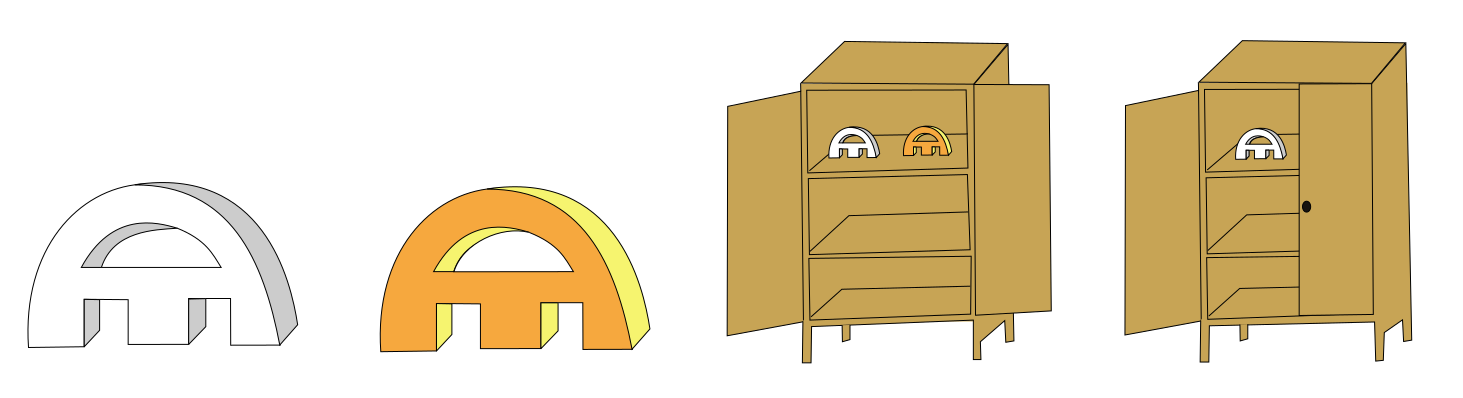
\includegraphics[width=0.5\textwidth]{figures/correanp1}
\caption{Ilustração do tipo de material usado com referente inanimado: \textit{Que depa sumiu?}}
\label{fig:correanp_1}
\end{figure}

A tarefa experimental exigia que a criança produzisse um DP fazendo referência a um dos objetos do mesmo tipo apresentado, distinguindo-o por meio de um adjetivo,\is{adjetivo} como \textit{A depa amarela} (ou simplesmente \textit{A amarela}), ou de forma dêitica, por meio de um pronome demonstrativo  \textit{Esta}/\textit{essa}/\textit{aquela depa} (ou simplesmente \textit{Esta}/\textit{essa}/\textit{aquela}). Logo, em todas as possíveis respostas verbais, o gênero\is{género} do pseudo-nome teria de ser codificado. O número de respostas em que o gênero\is{género} sinalizado pelo determinante\is{determinante} foi mantido (resposta-alvo) foi então tomado como informativo do quanto a criança tomaria a concordância\is{concordância} no DP como instrumento na identificação do gênero\is{género} de nomes\is{nome} novos.

Neste estudo, 30 crianças de 2;2 (2 anos e 2 meses) a 5;4 anos de idade foram divididas em dois grupos com idade média de 2;7 e 4;6.  A média das respostas-alvo foi consideravelmente alta em ambas as faixas etárias e apenas o grupo de crianças mais velhas foi impactado pela correlação entre a terminação do nome\is{nome} e o gênero\is{género} expresso no determinante,\is{determinante} com menor número de acertos na condição de não-congruência. Assim sendo, podemos constatar que a identificação do valor do traço sintático de gênero\is{género} em um elemento funcional,\is{elemento funcional} o D (tomado como núcleo do sintagma que define o domínio nominal) e sua atribuição ao nome,\is{nome} sob o pressuposto de que há concordância\is{concordância} entre os elementos do DP, permite que o gênero\is{género} intrínseco de nomes\is{nome} novos seja identificado desde tenra idade. Crianças mais velhas podem ser afetadas por um possível efeito de analogia, como sugerido com base em outras línguas, mas uma associação entre a forma do determinante\is{determinante} e a terminação do nome\is{nome} não é uma estratégia de aquisição.

O segundo estudo citado \citep{correa_etal2010} fez uso de seres inventados animados (Figura \ref{fig:correanp_2}).\footnote{Figura publicada originalmente em \citet{correa_etal2010}. Utilização autorizada pelos editores.} A criança era solicitada a contar o que tinha acontecido com o objeto/personagem no último quadrinho da tira, fazendo referência a este por meio de um DP definido pleno (Ex. \textit{O daba}), de um pronome pessoal (Ex. Ele) ou por meio de um demonstrativo (Ex Este). As variáveis manipuladas foram as mesmas do experimento anterior (gênero,\is{género} tal como informado pelo determinante)\is{determinante} e congruência entre o gênero\is{género} do determinante\is{determinante} e a terminação do pseudo-nome). 

Diante de nomes\is{nome} animados, o gênero\is{género} pode ser, em princípio, tanto intrínseco (tal como em o \textit{bode}, \textit{a ovelha}) quanto opcional (com nome\is{nome} flexionado em gênero,\is{género} tal como em o gato/a gat-a; ou invariável, como em o tenista/ a tenista). De qualquer forma, a informação confiável relativa ao gênero\is{género} está no determinante.\is{determinante} Tal como no estudo anterior, o número de respostas em que o gênero\is{género} expresso no determinante\is{determinante} é mantido foi tomado como indicativo do quanto essa informação foi tida como relevante para a criança. Se, contudo, nomes\is{nome} animados favorecem a expectativa de gênero\is{género} opcional e de que há flexão no nome,\is{nome} então, um efeito da incongruência entre determinante\is{determinante} e terminação do nome\is{nome} deveria ser esperado, particularmente no feminino, que é a forma marcada em gênero\is{género} pelo morfema \textit{–a}.

Os resultados foram semelhantes nas duas variedades do português. Nomes\is{nome} animados tenderam a ser tomados como de gênero\is{género} opcional pelas crianças, ou seja, nomes\is{nome} animados suscitaram o entendimento que categorias de gênero\is{género} podem definir classes conceituais. Os nomes\is{nome} masculinos tiveram maior número de respostas-alvo, o que sugere que o gênero\is{género} opcional feminino impõe maior demanda ao processamento e à aquisição da linguagem. Quando não havia congruência entre o gênero\is{género} feminino do determinante\is{determinante} e a terminação do nome,\is{nome} houve maior número de erros, particularmente no grupo de crianças mais novas. Também foi observado que a terminação do nome\is{nome} incongruente tendeu a ser alterada em função do gênero do determinante\is{determinante} (\textit{a depo para a depa}). A terminação em \textit{–a}, em nomes\is{nome} animados, parece, portanto, ser percebida como indicativa de flexão de gênero no nome.\is{nome} Crianças mais velhas tiveram melhor desempenho, particularmente no que diz respeito aos nomes\is{nome} femininos. 


Esses resultados revelam que, já aos 2 anos de idade, crianças diferenciam gênero\is{género} intrínseco de opcional. Cada um pode ser representado diferentemente em sua língua interna – o primeiro como uma propriedade do nome,\is{nome} o segundo como uma categoria funcional\is{categoria funcional} Gen, com a qual o nome\is{nome} concorda. De todo modo, tanto para o gênero\is{género} intrínseco quanto para o gênero\is{género} opcional, a criança toma a informação de gênero\is{género} do determinante\is{determinante} e parte do pressuposto de que há concordância\is{concordância} entre os elementos que compõem o DP.

No caso do número\is{número} gramatical, também é possível distinguir número\is{número} intrínseco (como em \textit{férias}, \textit{costas}, \textit{óculos}, \textit{calças} plural em PE)\footnote{Em PB, \textit{férias} tem número\is{número} intrínseco plural; coexistem as formas singular e plural \textit{o/os óculos}; e as formas plural as \textit{calças} e as \textit{costas} admitem a variação a calça e minha costa, em algumas variantes e/ou contextos.}, e número\is{número} opcional que, diferentemente do gênero,\is{género} é preponderante na língua. No caso do número\is{número} opcional, este varia em função do referente do DP (referente unitário, singular (\textit{um/o livro}); referente múltiplo, plural (\textit{um/uns livros})). Logo, assim como no gênero\is{género} opcional, pode-se assumir que uma categoria funcional\is{categoria funcional} Num, projetada como NumP, define o número\is{número} do DP \citep{ritter1991,augusto_etal2006}. 

Crianças que adquirem o PE encontram informação de número\is{número} no determinante\is{determinante} e em todos os elementos sintaticamente relacionados a este (nome,\is{nome} adjetivo).\is{adjetivo} Crianças que adquirem o PB encontram informação de número\is{número} necessariamente no determinante.\is{determinante} Dependendo da variante social /regional a que estejam predominantemente expostas terão maior ou menor contato com a expressão sistemática da concordância\is{concordância} nos demais elementos que compõem o DP. Em um estudo conduzido em PB, constatou-se que crianças expostas predominantemente à variante padrão, com idade média de 22 meses, interpretam, de forma semelhante, como DP plural, sintagmas como os dabos/ os dabo, em que o pseudo-nome apresenta-se flexionado e não flexionado.

A tarefa consistia na identificação de imagens correspondentes a um DP complemento de verbo, contendo um pseudo-nome, em um comando dado por um fantoche: \textit{Mostra os dabos pro Dedé!}  Esse comando foi variado de forma a criarem-se diferentes condições experimentais (i) DP com marca morfológica de plural (\textit{–s}) no D e no nome\is{nome} (forma padrão no PB e no PE), (ii) marca morfológica de plural apenas em D (variante atestada no PB), (iii) marca morfológica de plural apenas no nome\is{nome} (possível expressão de plural em línguas naturais, que é agramatical em PB e PE),\footnote{Ainda que agramatical, há evidência de produção desse tipo de expressão morfológica de número\is{número} na produção inicial de uma criança falante de PB, acompanhada dos 1;8 aos 3;2 anos de idade \citep{lopes2004,simioni2006}.} (iv) marca morfológica de plural apenas no interior do nome\is{nome} (infixo) (também agramatical no PB e PE). A forma singular foi usada como controle.

\ea\label{ex:correanp_19} Mostra \textit{os dabos/os dabo/o dabos/o dasbo/ o dabo} pro Dedé.
\z

O material visual apresentava 4 figuras: uma com mais de um objeto inventado (alvo da resposta decorrente da interpretação do DP como plural); duas com um objeto ou personagem inventado em cada uma, e outra com um objeto conhecido (como bola) (cf. Fig. \ref{fig:correanp_3}).

\begin{figure}
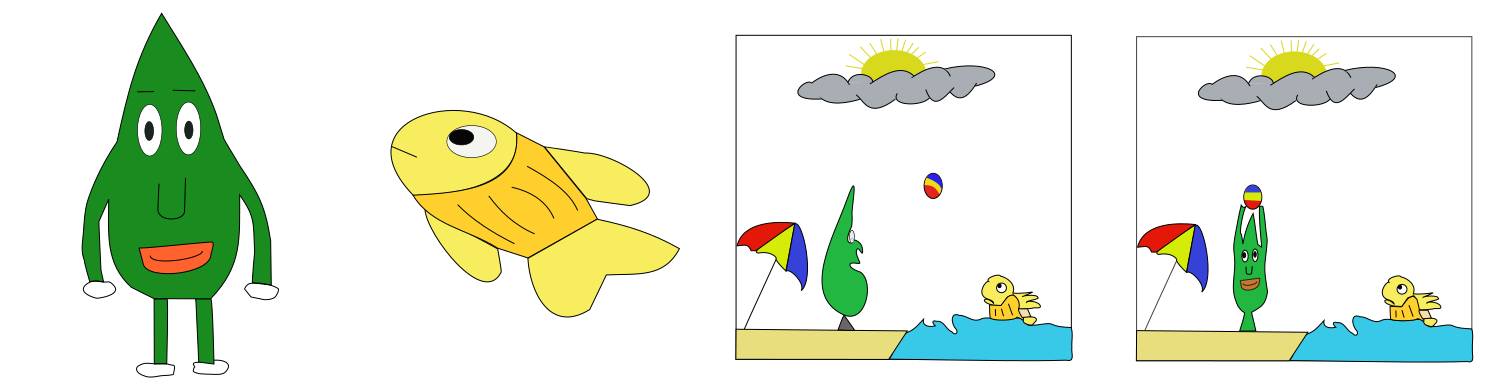
\includegraphics[width=0.5\textwidth]{figures/correanp2}
\caption{Ilustração do tipo de material usado com referente animado: \textit{Quem pegou a bola?}}
\label{fig:correanp_2}
\end{figure}

\begin{figure}
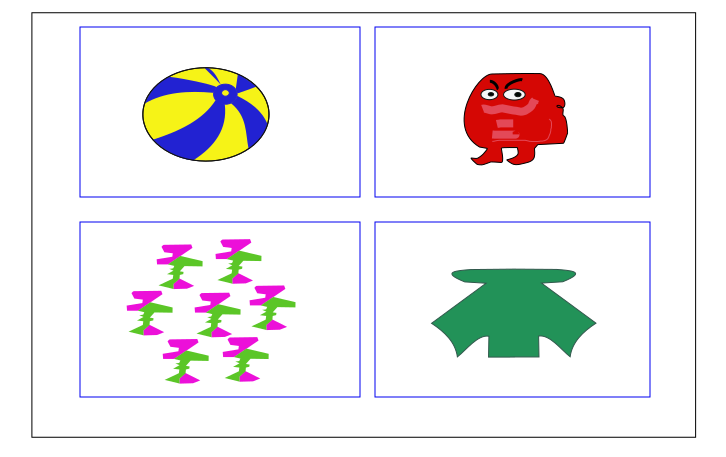
\includegraphics[width=0.5\textwidth]{figures/correanp3}
\caption{Ilustração do tipo de material utilizado em experimento sobre a compreensão de sintagmas no plural}
\label{fig:correanp_3}
\end{figure}

O experimento conduzido em PB \citep{correa_etal2005}, com 18 crianças com idade média de 22 meses, indicou que as crianças brasileiras são capazes de identificar a informação relativa a número\is{número} no DP, esteja esta expressa no determinante\is{determinante} e no nome,\is{nome} ou apenas no determinante\is{determinante} (61,1\% de acertos nas condições padrão e não-padrão do PB). A compreensão do DP plural mostrou-se mais custosa do que do singular (87,1\% de acertos). As formas agramaticais apresentaram percentuais de escolha da figura-alvo consideravelmente mais baixos. 

Este estudo foi replicado em PE \citep{castroferrarineto2007}, com 15 crianças (idade média de 26 meses).  Houve maior número de respostas-alvo (figura plural) na condição em que o morfema de plural está presente tanto no determinante\is{determinante} quanto no nome\is{nome} (76,6\%) em comparação com a marcação de plural exclusiva no determinante\is{determinante} (46,6\%).  De forma semelhante às crianças que adquirem o PB, um baixo número de respostas alvo foi obtido nas condições agramaticais.  Desse modo, o PE parece confirmar que D desempenha papel relevante para a identificação do número\is{número} gramatical e que, aos dois anos de idade, as crianças já reconheçam a forma redundante característica dessa variante da língua, como a realização do \isi{número} na língua em aquisição (\textit{o\textbf{s} dabo\textbf{s}}).

Em línguas como o inglês,\il{inglês} a expressão morfológica de número\is{número} no DP se apresenta no nome,\is{nome} em pronomes demonstrativos (\textit{This}/\textit{These}; \textit{That}/\textit{Those}) e quantificadores\is{quantificador} (\textit{some}; \textit{all}). Artigos são invariáveis.  Observa-se que a expressão do número\is{número} no DP, quando exclusiva no nome,\is{nome} acarreta dificuldade para crianças de dois anos, de forma razoavelmente independente da língua-alvo. 

Em experimento conduzido por meio da técnica da fixação preferencial do olhar, verificou-se que crianças que adquirem inglês\il{inglês} olham mais prontamente para o alvo quando a distinção singular-plural é expressa morfologicamente no verbo e no quantificador,\is{quantificador} além do nome.\is{nome} Ou seja, o mapeamento de \textit{blickets} em uma figura deu-se mais prontamente diante de instruções tais como \textit{Look, there are some blickets}/\textit{Look, there is a blicket}, do que \textit{Look at the blickets}/\textit{Look at the blicket} \citep{kouider_etal2006}. Assim sendo, a visibilidade da informação gramatical em elementos de uma categoria funcional\is{categoria funcional} parece contribuir para a sua identificação. 

É interessante observar que dados da produção da fala sugerem que a aquisição de número\is{número} no português é mais tardia do que os dados da compreensão sugerem. Em coleta longitudinal da produção de duas crianças de 24 a 28 meses, em aquisição do PB \citep{ferrarineto2003}, não foi encontrada evidência de marcação de número\is{número} em D. Evidência dessa marcação, em variante padrão e não padrão do PB, foi constatada na produção de uma criança a partir de 32 meses de idade \citep{simioni2006}.

Essa discrepância pode ser devida às demandas linguísticas e/ou cognitivas decorrentes da codificação da referência a elementos múltiplos na produção da fala. O uso de dados da percepção e da compreensão por parte de crianças em tenra idade são, portanto, particularmente reveladores de etapas iniciais do processo de especificação de informação pertinente ao domínio nominal da sintaxe.  Vimos que esse processo faz uso da percepção de informação sistemática (na morfologia), tomada como indicativa de informação gramaticalmente relevante assim como do pressuposto de que há concordância\is{concordância} entre os elementos que compõem o sintagma delimitado. 

\section{A aquisição de pessoa e a concordância sujeito-verbo}

Em português, assim como em várias línguas ocidentais, o verbo expressa concordância\is{concordância} de número\is{número} e pessoa\is{pessoa} com o DP sujeito. A aquisição de \textit{pessoa},\is{pessoa} como um traço formal (propriedade gramatical), em línguas em que se observa concordância\is{concordância} de pessoa\is{pessoa} e número\is{número} entre um DP sujeito e o verbo, irá requerer (i):  a identificação da variação de pessoa\is{pessoa} no DP sujeito – o que se realiza no sistema pronominal (1ª; 2ª e 3ª pessoa\is{pessoa} – em princípio, quem fala; com quem se fala; de quem se fala, com formas que podem variar em função de número);\is{número} e (ii) reconhecimento da expressão morfológica da concordância\is{concordância} sujeito e verbo, neste último. 

Em inglês,\il{inglês} por exemplo, a expressão da concordância\is{concordância} sujeito-verbo se reduz à forma –s na 3ª pessoa\is{pessoa} do singular de verbos em geral, no presente do indicativo (um tempo não marcado) e às variações na forma dos verbos \textit{be} e \textit{have}, que também atuam como auxiliares (1ª e 3ª pessoas\is{pessoa} do singular diferentes entre si e das demais pessoas,\is{pessoa} no presente e no passado no caso de \textit{be}; 3ª pessoa\is{pessoa} do singular do presente, no caso de \textit{have}), o que faz prever um processo relativamente custoso em relação a (ii) (ainda que a distinção da 1ª e da 3ª pessoas\is{pessoa} em verbos auxiliares possa facilitar seu reconhecimento).

Em línguas de morfologia rica, a criança pode, por outro lado, desde cedo perceber que raízes verbais não se apresentam de forma isolada na língua, como acontece no inglês.\il{inglês} Em italiano\il{italiano} e PE, por exemplo, há seis formas específicas para pessoa\is{pessoa}/número\is{número} acopladas ao verbo no presente do indicativo, sendo a 3ª pessoa\is{pessoa} do singular não marcada (\textit{-o}; \textit{-i}; \textit{-0}; \textit{-mo}; \textit{-te}; \textit{-no} (It.); \textit{-o}; \textit{-s}; \textit{-0}; \textit{-mos}; \textit{-is}; \textit{-m} (Port)). Considerando-se que as formas verbais regulares incluem uma vogal temática e podem ainda variar em tempo, aspecto e modo, a criança desde cedo pode perceber a impossibilidade de raízes verbais ocorrerem, sem que, pelo menos, a vogal temática a esta se acople (como na 3ª pessoa\is{pessoa} do singular, do presente do indicativo, ele cant\textit{-a}), o que pode ser um fator decisivo para o reconhecimento da expressão morfológica de concordância\is{concordância} sujeito-verbo na língua. 

Observa-se que, mesmo em muitas variedades do PB, em que o contraste número-pessoa\is{pessoa}\is{número} no verbo reduz-se a duas ou a quatro formas (1ª; 3ª pessoa;\is{pessoa} singular/plural), em comparação com a variedade padrão do PE (cf. Tabela \ref{tab:correanp}),\footnote{Maior incidência de formas tais como A\textit{ gente está}/\textit{estamos cansado}; \textit{A gente está}/\textit{estamos cansados}; \textit{A gente está}/e\textit{stamos cansada}; \textit{A gente está}/\textit{estamos cansadas} em PE do que em PB foi reportada em \citet{martoculio_etal2013} (cf. \citealt{vieirabrandao2014}).
} a criança pode, desde cedo, perceber que raízes verbais não se apresentam de forma isolada na língua, como acontece no inglês.\il{inglês} Em estudo conduzido por meio do paradigma da escuta preferencial com crianças que adquirem o PB, constatou-se que, por volta dos 10 meses de idade, crianças são capazes de perceber alterações fonológicas na morfologia verbal, em contraste com alterações semelhantes em raízes nominais, o que indica que já segmentam a forma verbal em raiz e afixos \citep{bagetticorrea2011}.

\begin{table}
\resizebox{\textwidth}{!}{
\begin{tabular}{lllp{5cm}}
\lsptoprule
Número                    & Pessoa                                 & Forma verbal -- PE         & Forma verbal -- PB                                                    \\ 
\midrule
\multirow{7}{*}{Singular} & \multirow{1}{*}{1ª EU}                 & \multirow{1}{*}{Cant-\textbf{\textit{o}}}    & Cant-\textbf{\textit{o}}                                                                \\ \cline{2-4}
                          & \multirow{3}{*}{2ª (direta) TU}                                       &                \multirow{3}{*}{Canta-\textbf{\textit{s}}}            & Canta-\textbf{\textit{s}} -- em poucas variedades                                       \\
                          &                                        &                            & Canta-\textbf{Ø} -- em variedades regionais e sociais, ou em registro informal \\
                          &                                        &                            & Ausente (substituída pela 2ª pessoa indireta)                          \\ \cline{2-4}
                          & 2ª (indireta) Você                     & Canta-\textbf{Ø}                    & Canta-\textbf{Ø} -- variante padrão e amplamente utilizada                     \\ \cline{2-4}
                          & 3ª Ele/Ela                             & Canta-\textbf{Ø}                    & Canta-\textbf{Ø}                                                               \\ \hline
\multirow{9}{*}{Plural}   & \multirow{2}{*}{1ª Nós}                & \multirow{2}{*}{Canta-\textbf{\textit{mos}}} & Canta-\textbf{\textit{mos}} -- variante padrão                                          \\
                          &                                        &                            & Canta-\textbf{Ø} -- variante não-padrão                                        \\ \cline{2-4}
                          & \multirow{2}{*}{1ª (informal) A gente} & Canta-\textbf{Ø}                    & Canta-\textbf{Ø}                                                               \\
                          &                                        & Cant-\textbf{\textit{amos}}                  & Cant-\textbf{\textit{amos}} -- variante não padrão                                      \\ \cline{2-4}
                          & 2ª (direta) Vós                        & Canta-\textbf{\textit{is}}                   & Ausente                                                               \\ \cline{2-4}
                          & \multirow{2}{*}{2ª (indireta) Vocês}   & \multirow{2}{*}{Canta-\textbf{\textit{m}}}   & Canta-\textbf{\textit{m}} -- variante padrão                                            \\
                          &                                        &                            & Canta-\textbf{Ø} -- variante não padrão                                        \\ \cline{2-4}
                          & \multirow{2}{*}{3ª Eles/Elas}          & \multirow{2}{*}{Canta-\textbf{\textit{m}}}   & Canta-\textbf{\textit{m}} -- variante padrão                                            \\
                          &                                        &                            & Canta-\textbf{Ø} -- variante não-padrão \\
\lspbottomrule
\end{tabular}}
  \caption{Realização morfológica de pessoa e número no verbo em variedades do português}
  \label{tab:correanp}
\end{table}

Diante das variações entre línguas, seria esperado que as distinções de pessoa\is{pessoa}/número\is{número} como expressão de concordância\is{concordância} no verbo fossem mais prontamente identificadas em línguas de morfologia rica do que em línguas com poucas distinções morfológicas, como o inglês.\il{inglês} Dados da aquisição da linguagem sugerem ser este o caso.

No inglês,\il{inglês} crianças de 19 meses estranham a ausência da expressão de concordância,\is{concordância} \textit{-s} no verbo (possivelmente em função de sua considerável recorrência) \citep{soderstrom_etal2002}. O uso produtivo da marca de concordância\is{concordância} em verbos desconhecidos pode ser constatado em crianças de 2;6 meses a 3 anos, em estudo que fez uso de treinamento \citep{theakston_etal2003}. É, contudo, apenas aos 4 anos de idade que o número de ocorrências do morfema de 3ª pessoa\is{pessoa} singular em contexto obrigatório parece alcançar 90\% das respostas em tarefa de produção elicitada \citep{ricewexler2002}, o que tem certa correspondência com a ocorrência do morfema de plural no nome,\is{nome} nos dados de Brown (Estádios IV e V – a partir de 3;5 anos) \citep{brown1973}.

Dados da produção espontânea de crianças que adquirem o italiano,\il{italiano} por sua vez, revelam que a morfologia verbal de pessoa\is{pessoa} singular no presente do indicativo aparece no que seriam os Estádios I e II de Brown. Na aquisição do PE, o contraste entre primeira e terceira pessoa\is{pessoa} do singular na concordância\is{concordância} sujeito-verbo foi constatado na fala de crianças de 1;10 a 2;7 meses \citep{goncalves2004}, novamente bem antes do que se observa no inglês.\il{inglês} No que concerne ao PB, um estudo longitudinal de duas crianças revelou que após um período de flutuação entre a concordância\is{concordância} entre DP-sujeito e verbo, o contraste entre 1ª e 3ª pessoa\is{pessoa} torna-se estável aos 23 meses (1;11 meses) \citep{martins2007}.

Nem sempre, contudo, evidência de concordância\is{concordância} na fala implica que a criança tenha habilidade de fazer uso exclusivo da informação veiculada na desinência verbal na interpretação da sentença. Em estudo conduzido em inglês\il{inglês} \citep{johnson_etal2005}, estímulos do tipo \textit{Show me the picture where\ldots the duck swim (\textbf{-s}) in the water} foram utilizados. Note-se que o número\is{número} gramatical do sujeito fica indiferenciado pelo fato de o verbo ter \textipa{/s/} como a consoante inicial (\textit{the ducks wim ou the duck swim}). Assim sendo, é a presença do morfema \textit{–s} no verbo que dissolve a ambiguidade. Os resultados sugerem que apenas aos 5--6 anos de idade, crianças atentam para a pessoa\is{pessoa} do verbo como fonte de informação para o número\is{número} do sujeito.

Em experimento conduzido em português, com crianças em processo de aquisição de PB, buscou-se verificar em que elemento do par DP-verbo a informação de pessoa\is{pessoa} estaria mais saliente \citep{martins2007,correamartins2008}. Para isso, 26 crianças de 3 e de 5 anos participaram de uma tarefa em que deveriam entregar um brinquedo a um de dois fantoches, com base no que eles diziam, e foram alertadas de que eles não sabiam falar muito bem. 

Quatro condições experimentais foram criadas em função da manipulação de pessoa\is{pessoa} (1ª e 3ª) e de congruência entre DP e verbo (congruente, quando a forma verbal corresponde à pessoa\is{pessoa} expressa no DP sujeito; incongruente, quando para sujeito em 1ª pessoa\is{pessoa} tem-se a forma verbal da 3ª pessoa\is{pessoa} e vice-versa). Por exemplo, nas condições congruentes, um fantoche dizia \textit{Eu quero esse carro} ou \textit{Ele quer esse carro}, para que a criança entregasse um carrinho a um dos dois fantoches. Nas condições incongruentes, o fantoche dizia \textit{Eu quer esse carro} ou \textit{Ele quero esse carro}. 

Considerou-se como resposta-alvo aquela em que a criança entrega o brinquedo ao fantoche referente do DP sujeito (\textit{eu}, para o que fala; \textit{ele} para o outro). Os resultados revelaram que as condições congruentes, como pode ser antecipado, têm maior número de respostas-alvo, que aumenta com a idade. Quanto ao efeito de pessoa,\is{pessoa} a 1ª pessoa\is{pessoa} mostrou-se mais fácil de ser interpretada do que a 3ª, tanto nas condições congruentes quanto nas incongruentes, possivelmente devido a seu caráter dêitico e à disponibilidade dessa informação na terminação do verbo flexionado. A condição \textit{Eu quer}, teve um alto número de respostas-alvo, o que indica que \textit{pessoa}\is{pessoa} foi interpretada no DP sujeito, admitindo-se a forma não marcada (ou \textit{default}) do verbo. Já a condição \textit{Ele quero} mostrou-se a mais difícil, com respostas-alvo no nível de chance mesmo no grupo de 5 anos. A expressão morfológica de 1ª pessoa\is{pessoa} no verbo é, portanto, tão informativa quanto o pronome-sujeito \citep{martins2007,correamartins2008}. 

Em suma, DPs codificam informação necessária ao estabelecimento da referência – pessoa\is{pessoa} (do discurso), número\is{número} opcional, gênero\is{género} opcional, assim como informação pertinente à classificação de nomes em classes de gênero.\is{género} A identificação de traços opcionais (que remetem a propriedades do referente do DP) deve acarretar a representação de categorias funcionais\is{categoria funcional} específicas, como GenP e NumP. A criança torna-se sensível às variações morfológicas sinalizadoras de concordância\is{concordância} no âmbito do DP e das relações sujeito-verbo e busca interpretá-las sob o pressuposto de que itens lexicais relacionados estruturalmente em sintagmas compartilham traços. O processo de aquisição do que há de específico na língua requer, portanto, que operações sintáticas sejam postas em execução tão logo os elementos do léxico em constituição possam ser diferenciados em funcionais (classe fechada)\is{classe fechada} e lexicais (classe aberta).\is{classe aberta}

\section{A expressão morfológica da concordância\is{concordância} no caso de perturbação da linguagem}
\label{sec:correanp_expressao}

A expressão morfológica da concordância no DP mostra-se reveladora no que diz respeito ao comprometimento linguístico em crianças, particularmente ao que vem sendo denominado \textit{Perturbação Específica da Linguagem}\is{Perturbação Específica da Linguagem} (PEL - em Portugal) ou Déficit/Distúrbio Específico da Linguagem (DEL - no Brasil),\is{Distúrbio Específico da Linguagem|see {Perturbação Específica da Linguagem}} correspondentes a \textit{Specific Language Impairment}\is{Specific Language Impairment|see {Perturbação Específica da Linguagem}} (SLI) do inglês.\il{inglês} Essa condição caracteriza-se por um comprometimento no nível da linguagem que pode afetar apenas a produção ou ambas modalidades, produção e compreensão, sem que haja qualquer outro comprometimento de nível cognitivo, neurológico ou psicológico, que possa justificar o atraso linguístico \citep{leonard1995}. O tipo de comprometimento apresentado varia de criança para criança, podendo afetar uma ou mais áreas da linguagem: léxico, fonologia, morfossintaxe ou pragmática \citep{friedmannnovogrodsky2008}.

No que diz respeito a manifestações de PEL/DEL no âmbito do DP, a ausência ou  opcionalidade da morfologia referente a gênero,\is{género} número\is{número} e pessoa\is{pessoa} tem sido reportada. A omissão de determinantes\is{determinante} também tem sido observada com mais frequência em crianças com suspeita ou diagnóstico de PEL/DEL do que aquelas com desenvolvimento típico (\citealt{leonard1995} – inglês;\il{inglês} \citealt{roulet2007} – francês;\il{francês} \citealt{bortolini_etal1997} – italiano;\il{italiano} \citealt{branco_etal2011} - PE; \citealt{silveira2002,silveira2006} - PB). Em termos dos erros de concordância\is{concordância} de gênero\is{género} e número\is{número} no DP, emissões atípicas são reportadas, particularmente em línguas românicas, de morfologia rica, embora omissões do sufixo \textit{–s} que marca a forma plural também sejam comuns em inglês\il{inglês} \citep{leonard1995}. Abaixo encontram-se alguns exemplos de alterações morfossintáticas sugestivas de PEL/DEL no português \citep{castrogomes2000,haeusler2005}:

\ea\label{ex:correanp_20} Est\textbf{e} escada é muito alt\textbf{o} (D., 4 anos)\z
\ea\label{ex:correanp_21} Esta é mais pequenin\textbf{o} (D., 4 anos)\z
\ea\label{ex:correanp_22} uma porca gordo\z
\ea\label{ex:correanp_23} O dois casas (D., 4 anos)\z

Para o PB, uma bateria de testes acerca da concordância\is{concordância} de gênero\is{género} foi aplicada a um grupo de seis crianças com suspeita de PEL/DEL \citep{silveira2006}, cujos resultados indicam que o desempenho das crianças com comprometimento é, de maneira geral, pior que o das crianças com desenvolvimento típico, emparelhadas por idade, embora haja no grupo experimental alta variabilidade nos resultados individuais. Quanto a \textit{número},\is{número} onze crianças com suspeita de PEL/DEL falantes de PB foram testadas em tarefas de compreensão com nomes\is{nome} e pseudo-nomes\is{nome} flexionados e não-flexionados em número,\is{número} com e sem adjetivos.\is{adjetivo} Seu desempenho foi inferior ao das crianças com desenvolvimento típico, sendo que a presença do adjetivo\is{adjetivo} pareceu dificultar ainda mais a tarefa para o grupo de crianças com comprometimento \citep{bomfim2008}.

Em PE, um grupo de oito crianças com diagnóstico ou suspeita de PEL/DEL foi exposto, no que concerne à concordância\is{concordância} de gênero\is{género} e de número\is{número} no DP, a tarefas de compreensão e de produção \citep{branco_etal2011}. Para compreensão, foi utilizada a técnica de seleção de imagens com uso de pseudo-nomes para objetos inventados (adaptada de \citealt{correa_etal2010}). Na produção elicitada, foram utilizados nomes\is{nome} e pseudo-nomes (adaptada de \citealt{silveira2006}). Os resultados vão na mesma direção daqueles obtidos no PB, indicando-se uma maior dificuldade frente a nomes\is{nome} novos e salientando-se uma considerável variabilidade individual nos resultados.

De maneira geral, os resultados parecem indicar que, embora o desempenho de crianças com PEL/DEL indique problemas tanto com gênero\is{género} quanto com número,\is{número} isso não significa que os valores desses traços não tenham sido identificados. No entanto, não é claro em que medida o procedimento de aquisição dessa informação linguística é semelhante ao de crianças com desenvolvimento típico, ou seja, com base no pressuposto de que há concordância\is{concordância} entre elementos sintaticamente relacionados. 

Em relação à flexão de pessoa\is{pessoa}/número\is{número} no verbo, dados do inglês\il{inglês} indicam a presença regular de formas infinitivas e omissão do morfema da terceira pessoa\is{pessoa} do singular \textit{–s}. Essa ausência ou opcionalidade de marcas morfológicas de concordância\is{concordância} no verbo são também atestadas no alemão\il{alemão} \citep{clahsen_etal1997}. 

Em PB, uma investigação conduzida com duas crianças com suspeita de PEL/DEL, nos moldes de \citet{correamartins2008}, apresentado na seção anterior, verificou que essas crianças apresentavam dificuldades na compreensão de informação relativa à 3ª pessoa,\is{pessoa} particularmente à 3ª pessoa\is{pessoa} do plural, ainda que com idade superior a 5 anos.

O processo de aquisição e de acesso à informação gramatical relativa a propriedades definidoras do domínio nominal (gênero,\is{género} número\is{número} e pessoa),\is{pessoa} encontram-se, portanto, vulneráveis em casos sugestivos de PEL/DEL. 

\section{Para concluir}
\label{sec:correanp_conclusao}

O tradicional sintagma nominal\is{sintagma nominal} (SN), hoje caracterizado como sintagma determinante\is{sintagma determinante}\is{determinante} (DP), em teorias generativistas, é peça crucial para a referência, sendo fundamental para a expressão do pensamento na relação entre linguagem e mundo. Na aquisição da linguagem, cabe à criança identificar o que há de específico dos constituintes nominais da língua e de sua relação com outros constituintes da oração. Vimos que a aquisição de informação gramatical pertinente ao domínio nominal tem início em tenra idade, que ao fim do primeiro ano de vida, constituintes nominais já são reconhecidos pela criança, mas que o processo de aquisição irá requerer a progressiva especificação de propriedades sintáticas no léxico em aquisição. Buscamos explicar esse processo como decorrente de uma faculdade de linguagem que possibilita o reconhecimento de padrões recorrentes nos dados da fala como informação gramaticalmente relevante e o uso de operações sintáticas comuns às línguas humanas como instrumento para a identificação das propriedades específicas relativas a gênero,\is{género} número\is{número} e pessoa,\is{pessoa} que são os traços sintáticos característicos do domínio nominal da língua. 

\section*{Nota}

Este capítulo foi elaborado durante a vigência do projeto 308874/2011-0 (PQ-CNPq)  (Conselho Nacional de Desenvolvimento Científico e Tecnológico), da primeira autora.





{\sloppy
\printbibliography[heading=subbibliography,notkeyword=this]
}
\end{document}